\def\pgfsysdriver{pgfsys-dvisvgm.def}
\documentclass[dvisvgm,tikz,border=10pt]{standalone}
\usepackage{tikz}
\usepackage{amsmath}
\usetikzlibrary{arrows.meta,patterns,positioning}
\tikzset{
 clause/.style={rectangle,draw=black,fill=white,minimum size=7mm,line width=.9pt},
 varnode/.style={circle,draw=black,minimum size=9mm,line width=.9pt},
 truevar/.style={varnode,fill=white},
 falsevar/.style={varnode,fill=gray!55},
 freevar/.style={varnode,pattern=north east lines,pattern color=gray!65},
 positive/.style={draw=black,line width=1pt},
 negative/.style={positive,dash pattern=on 4pt off 3pt},
 every node/.style={text=black,font=\sffamily},
}

\begin{document}
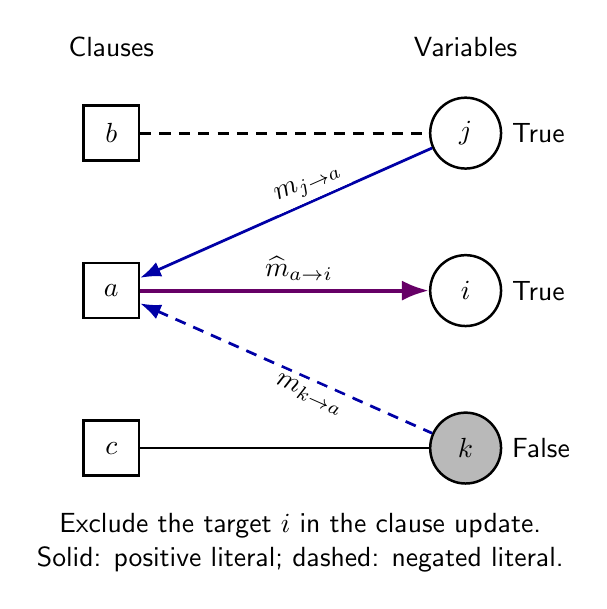
\begin{tikzpicture}
\node at (0,3.1) {Clauses}; \node at (4.5,3.1) {Variables};
\node[clause] (b) at (0,2) {$b$};
\node[clause] (a) at (0,0) {$a$};
\node[clause] (c) at (0,-2) {$c$};
\node[truevar,label=right:True] (j) at (4.5,2) {$j$};
\node[truevar,label=right:True] (i) at (4.5,0) {$i$};
\node[falsevar,label=right:False] (k) at (4.5,-2) {$k$};
\draw[negative] (b)--(j);
\draw[positive] (c)--(k);
\draw[positive,draw=blue!65!black,{Latex}-] (a)--
 node[pos=.6,above,sloped,fill=white,inner sep=2pt] {$m_{j\to a}$} (j);
\draw[negative,draw=blue!65!black,{Latex}-] (a)--
 node[pos=.6,below,sloped,fill=white,inner sep=2pt] {$m_{k\to a}$} (k);
\draw[positive,draw=violet!80!black,-{Latex},line width=1.5pt] (a)--
 node[pos=.55,above,fill=white,inner sep=3pt] {$\widehat m_{a\to i}$} (i);
\node[align=center] at (2.4,-3.2) {Exclude the target $i$ in the clause update.\\
Solid: positive literal; dashed: negated literal.};
\end{tikzpicture}
\end{document}
